\documentclass[aspectratio=169]{beamer}
\usepackage[utf8]{inputenc} % codificacao de caracteres
\usepackage[T1]{fontenc}    % codificacao de fontes
\usepackage[brazil]{babel}  % idioma
\usepackage{graphics,amssymb,amsfonts,amsmath}
\usepackage{tikz}
\usepackage{enumerate,hyperref}
\usepackage{palatino}	% Fonte sem serifa
\usepackage{ragged2e}	% Paragrafo justificado
%\usepackage{minted}	% Highlight para codigos de programacao
\usepackage{booktabs} % tabelas
\usepackage{multicol}
\usepackage{multirow}
%\usepackage[table]{xcolor}


% Veja mais temas e cores em http://www.hartwork.org/beamer-theme-matrix/
\usetheme{Montpellier}         % tema
\usecolortheme{orchid}      % cores
\usefonttheme[onlymath]{serif} % fonte modo matematico
% Colocando numero de paginas no slide
\setbeamertemplate{footline}[frame number]



\DeclareGraphicsExtensions{.pdf,.jpg,.png} % compilamos apenas com pdflatex
\graphicspath{{./figuras/}} % caminho onde as figuras estarao disponiveis




% ---------------------------------------------------------------------------- %
% T�tulo                                                                       %
% ---------------------------------------------------------------------------- %

\title[\sc{Teoria de Circuitos Eletrônicos 1}]{\LARGE Aula 2: Methods of Analysis of Resistive Circuits (Node Voltage)}
\author[Prof. Marcelino Andrade]{Prof. Marcelino Andrade}
\institute{Faculdade UnB Gama} % opcional
\date{\today}

\begin{document}
\justifying % Paragrafo justificado
\pagebreak

\begin{frame}
  \titlepage
\end{frame}


% ----------------- NOVO SLIDE --------------------------------
\begin{frame}{Contents\newline}

\tableofcontents
\begin{center}	
     		Introduction to Electric Circuits 9th Edition by James A. Svoboda, Richard C. Dorf			
\end{center}	
\end{frame}

% ----------------- NOVA SECÇÂO -----------------------------
\section{Introduction (4.1)}
% ----------------- NOVO SLIDE --------------------------------
\begin{frame}[fragile]
	\frametitle{Introduction}
		\begin{tabular}{cc}
			\begin{columns}
				\begin{column}{1\textwidth}  %%<--- here
					In this chapter, we consider two methods for writing a smaller set of simultaneous equations:	\newline
		
					\begin{itemize}
						\item[$\clubsuit$] \scalebox{1.5}{The node voltage method.}
						\item[$\clubsuit$] \scalebox{1.5}{The mesh current method.}						
					\end{itemize}
					.\newline To analyze an electric circuit, we write and solve a set of equations. We apply Kirchhoff’s current and
					voltage laws to get some of the equations. This method works well for small circuits, but the set of equations can get quite large for even
					moderate-sized circuits.
				\end{column}
			\end{columns}
		
	\end{tabular}
\end{frame}
% ----------------- NOVO SLIDE --------------------------------

% ----------------- NOVA SECÇÂO -----------------------------
\section{Node Voltage Analysis of Circuits with Current Sources (4.2)}
% ----------------- NOVO SLIDE --------------------------------
\begin{frame}[fragile]
	\frametitle{Node Voltage Analysis of Circuits with Current Sources}

\begin{tabular}{ll}
	\begin{columns}
		\begin{column}{0.3\textwidth}  %%<--- here
    			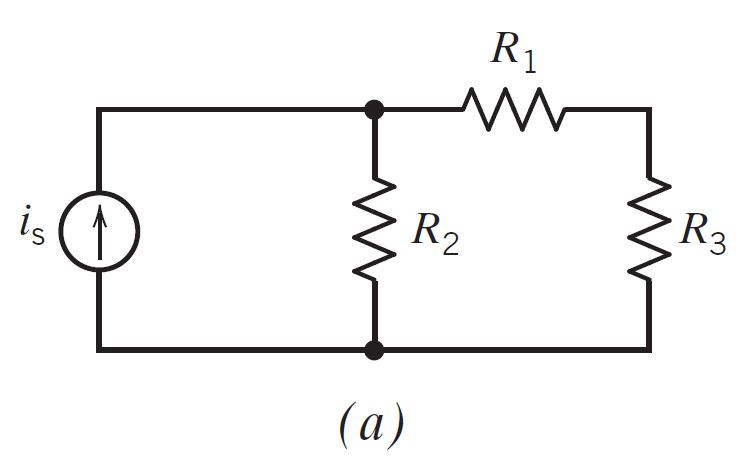
\includegraphics[width=0.9\textwidth]{figura4_21a.jpg}\\	
			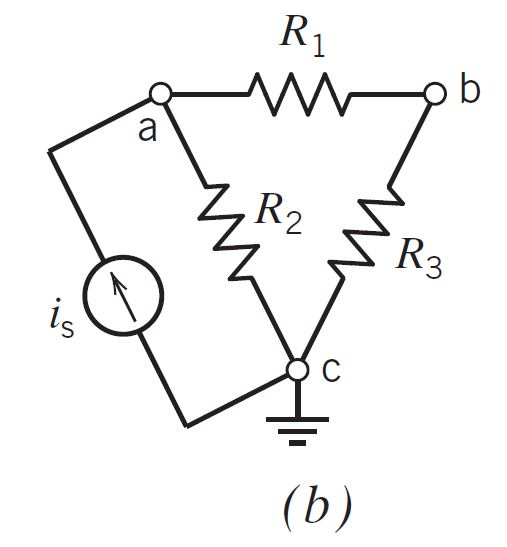
\includegraphics[width=0.9\textwidth]{figura4_21b.jpg} \\	
			
		\end{column}
		\begin{column}{0.7\textwidth}  %%<--- here
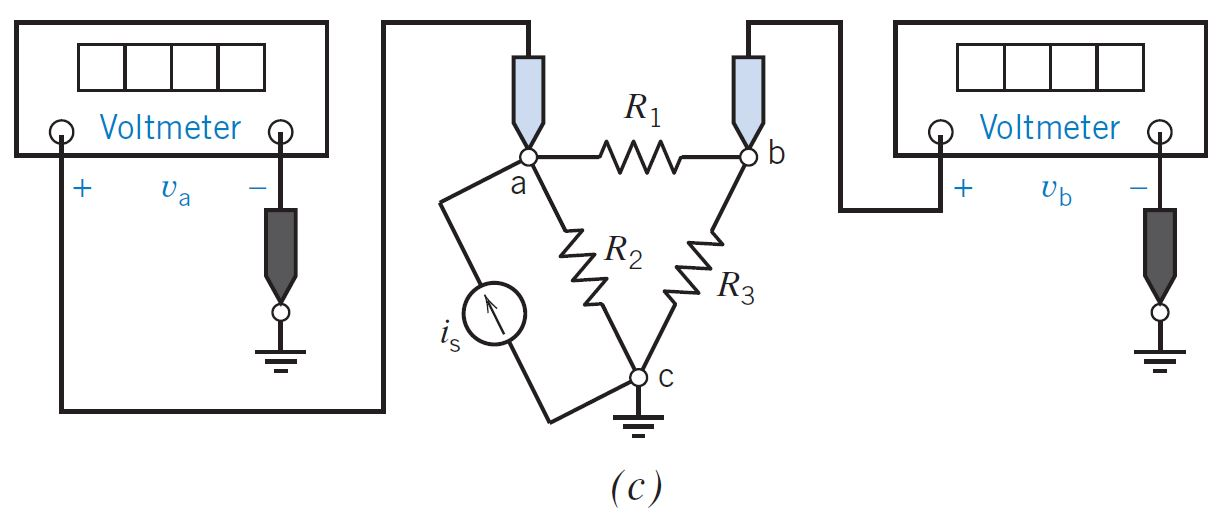
\includegraphics[width=.8\textwidth]{figura4_21c.jpg}\\	
					\begin{enumerate}[(a)]
						\item {A circuit with three nodes.}
						\item {The circuit with nodes labeled and reference node marked.}
						\item {Using voltmeters to measure the node voltages.}							
					\end{enumerate}

					
		\end{column}
	\end{columns}
\end{tabular}



\end{frame}
% ----------------- NOVO SLIDE --------------------------------
\begin{frame}[fragile]
	\frametitle{The Node Voltage}

\begin{tabular}{ll}
	\begin{columns}
		\begin{column}{0.3\textwidth}  %%<--- here
    			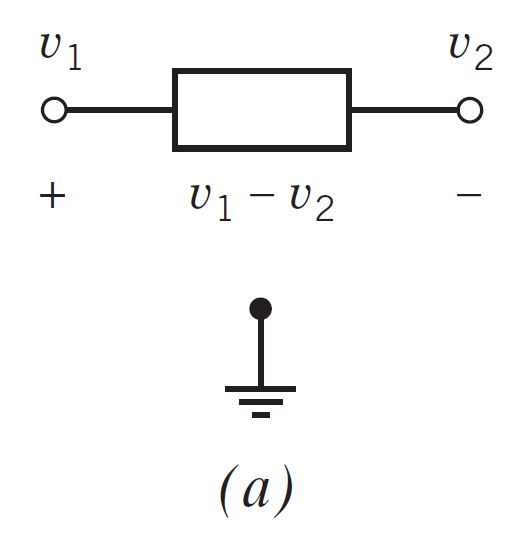
\includegraphics[height=.9\textwidth]{figura4_23a.jpg}\\	
			Generic element
		\end{column}
		\begin{column}{0.3\textwidth}  %%<--- here
			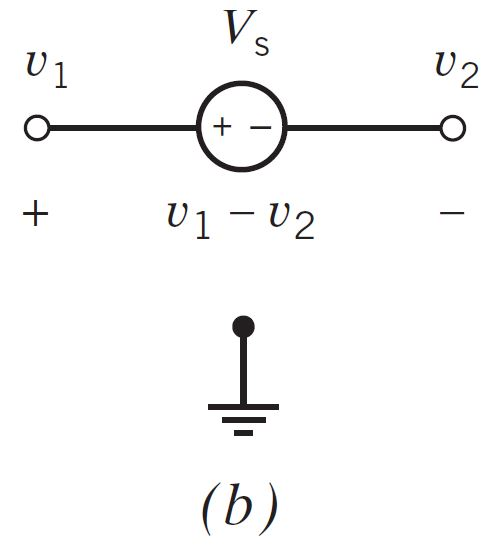
\includegraphics[height=.9\textwidth]{figura4_23b.jpg}\\	
			Voltage source
		\end{column}
		\begin{column}{0.3\textwidth}  %%<--- here
			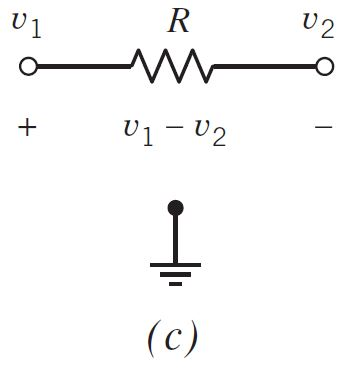
\includegraphics[height=.9\textwidth]{figura4_23c.jpg}\\	
			Resistor
		\end{column}




	\end{columns}
\end{tabular}
\end{frame}
% ----------------- NOVO SLIDE --------------------------------

\begin{frame}[fragile]
	\frametitle{The Node Equations}

\begin{tabular}{ll}
	\begin{columns}
		\begin{column}{0.4\textwidth}  %%<--- here
    			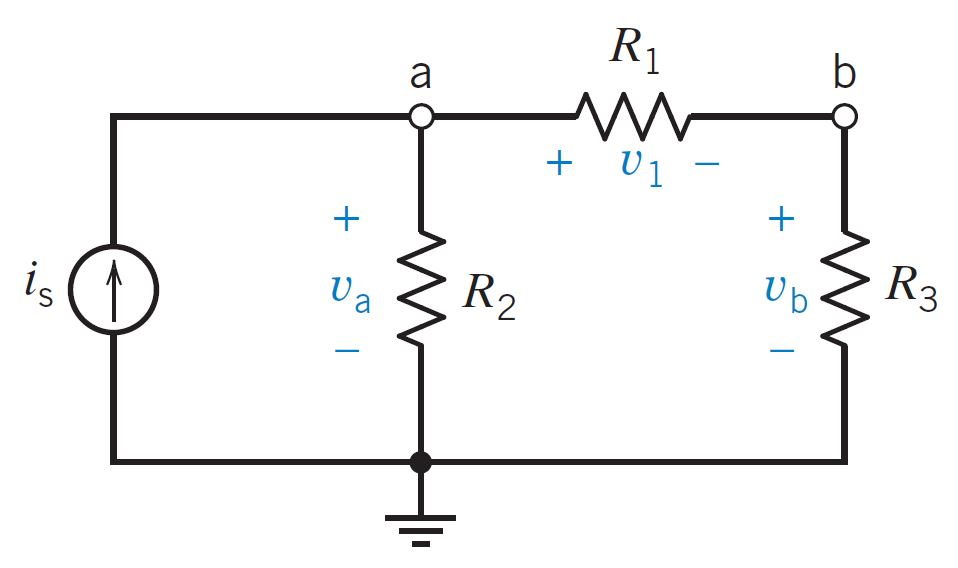
\includegraphics[width=1\textwidth]{figura4_24.jpg}\\	

		\end{column}
		\begin{column}{0.6\textwidth}  %%<--- here


{To write a set of node equations, we do two things:}\\

					\begin{itemize}
						\item[$\clubsuit$] {Express element currents as functions of the node voltages.}
						\item[$\clubsuit$]  {Apply Kirchhoff’s current law (KCL) at each of the nodes of the circuit except for the reference node.}
						
					\end{itemize}
		\end{column}
		




	\end{columns}
\end{tabular}
\end{frame}
% ----------------- NOVO SLIDE --------------------------------

\begin{frame}[fragile]
	\frametitle{Node Voltage Analysis}

\

\begin{tabular}{ll}
	\begin{columns}[c]	\column{1\textwidth}
		\textbf{ EXAMPLE 4.2-2} - Obtain the node equations for the circuit.\\
\begin{center}
{}
\end{center}
	\end{columns} \\
	\begin{columns}
		\begin{column}{0.4\textwidth}  %%<--- here
		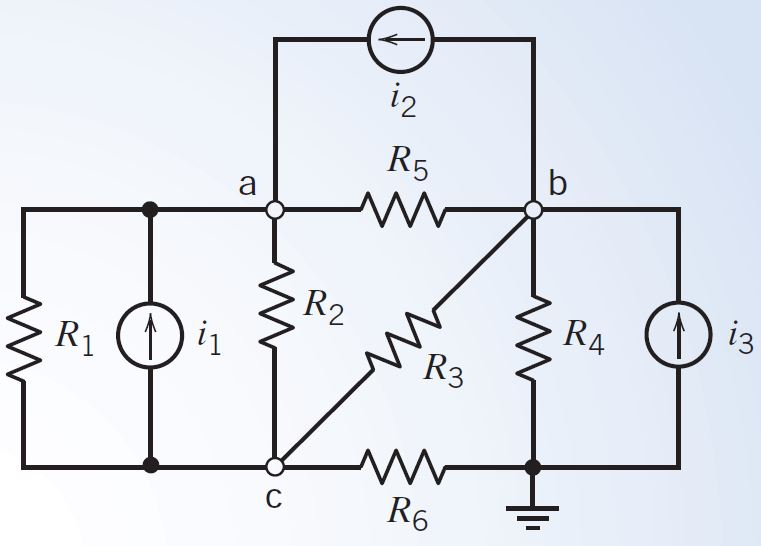
\includegraphics[width=1.1\textwidth]{figura4_26.jpg}\\	
	%	\scalebox{1}{Answer:$\ v_{a} = -4/3V\ and \  v_{b} = 4 V$}
		\end{column}
		\begin{column}{0.6\textwidth}  %%<--- here
			\[ 
			\left[\begin{array}{ccc}
			\frac{1}{R_{1}}+\frac{1}{R_{2}}+\frac{1}{R_{5}} & -\frac{1}{R_{5}} & -(\frac{1}{R_{1}}+\frac{1}{R_{2}})\\
			-\frac{1}{R_{5}} & \frac{1}{R_{3}}+\frac{1}{R_{4}}+\frac{1}{R_{5}} & -\frac{1}{R_{3}} \\
			-(\frac{1}{R_{1}}+\frac{1}{R_{2}}) & -\frac{1}{R_{3}} & \frac{1}{R_{1}}+\frac{1}{R_{2}}+\frac{1}{R_{3}}+\frac{1}{R_{6}} \end{array} \right] \] \\ \[ \times\
			\left[\begin{array}{c}
			v_{a} \\
			v_{b} \\
			 v_{c}\end{array} \right]= 
			\left[\begin{array}{c}
			i_{1}+i_{2} \\
			i_{3}-i_{2} \\
			-i_{1}  \end{array} \right]
			\]	
		\end{column}
	\end{columns}\\

\end{tabular}


\end{frame}
















% ----------------- NOVO SLIDE --------------------------------

\begin{frame}[fragile]
	\frametitle{Node Voltage Analysis}

\begin{tabular}{ll}
	\begin{columns}
		\begin{column}{1\textwidth}  %%<--- here
		\textbf{EXERCISE 4.2-2} - Determine the node voltages $v_{a}$ and $v_{b}$ for the circuit.\\
		\begin{center}
    			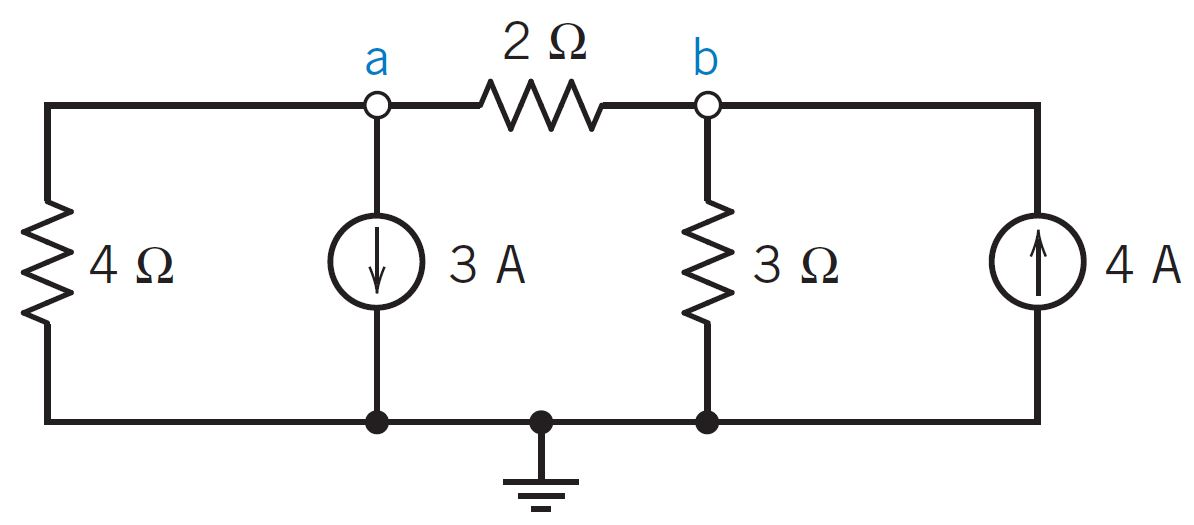
\includegraphics[width=.65\textwidth]{figuraE4_22.jpg}\\	
		\end{center}	
		\scalebox{0.8}{Answer:$\ v_{a} = -4/3V\ and \  v_{b} = 4 V$}
		\end{column}
	\end{columns}
\end{tabular}
\end{frame}






% ----------------- NOVA SECÇÂO -----------------------------
\section{Node Voltage Analysis of Circuits with Current and Voltage Sources (4.3)}
% ----------------- NOVO SLIDE --------------------------------
\begin{frame}[fragile]
	\frametitle{Node Voltage Analysis of Circuits with Current and Voltage Sources}
\begin{tabular}{ll}
	\begin{columns}[c]	\column{1\textwidth}
		First we consider the circuit with a voltage source between ground and one of the other nodes.
	\end{columns} \\
	\begin{columns}
		\begin{column}{0.6\textwidth}  %%<--- here
		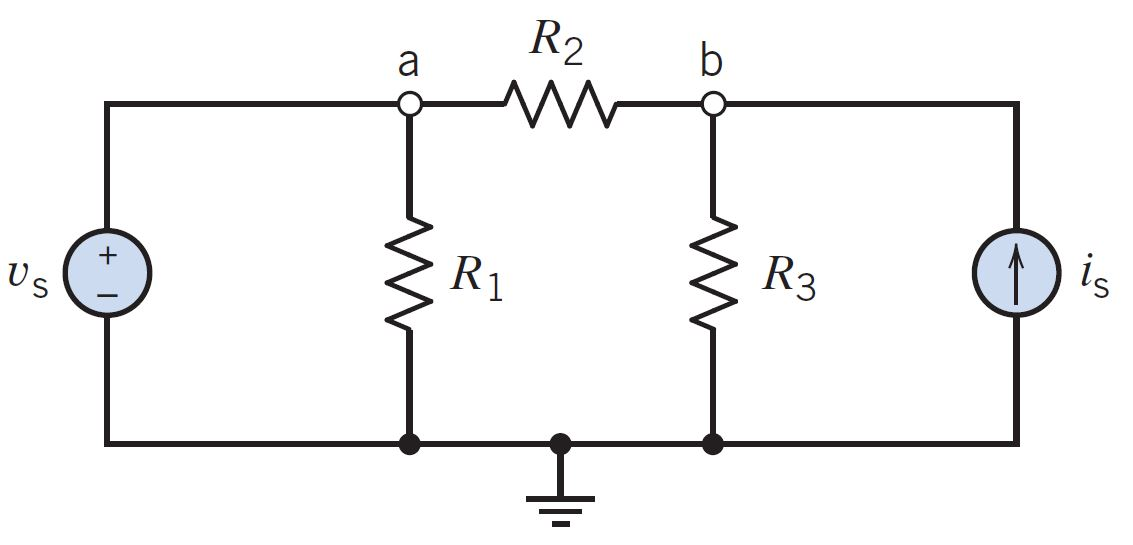
\includegraphics[width=1\textwidth]{figura4_22.jpg}\\	
	%	\scalebox{1}{Answer:$\ v_{a} = -4/3V\ and \  v_{b} = 4 V$}
		\end{column}
		\begin{column}{0.4\textwidth}  %%<--- here
			\begin{equation}
			 v_{a}= v_{s}
			\end{equation}
			\begin{equation}
			- i_{s}+\frac{ v_{b}}{R_{3}}+\frac{ v_{b}-v_{a}}{R_{2}}=0
			\end{equation}
			\begin{equation}
			 -i_{s}+\frac{ v_{b}}{R_{3}}+\frac{ v_{b}-v_{s}}{R_{2}}=0
			\end{equation}
			\begin{equation}
			 v_{b}=\frac{ R_{2}R_{3}i_{s}+R_{3}v_{s}}{R_{2}+R_{3}}
			\end{equation}
		\end{column}
	\end{columns}
\end{tabular}
\end{frame}
% ----------------- NOVO SLIDE --------------------------------
\begin{frame}[fragile]
	\frametitle{Node Equations}

\begin{tabular}{ll}
	\begin{columns}
		\begin{column}{1\textwidth}  %%<--- here
		\textbf{EXAMPLE 4.3-1} - Determine the values node voltages, $v_{1}$ and $v_{2}$, in the circuit.\\
		\begin{center}
    			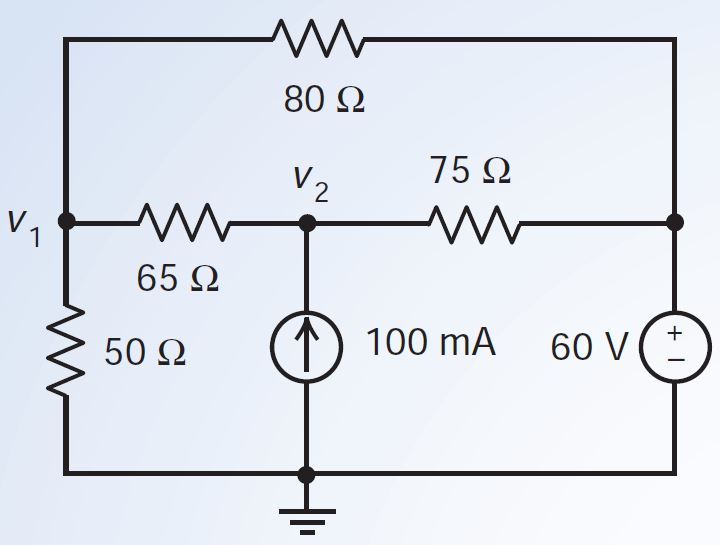
\includegraphics[width=.35\textwidth]{figura4_33.jpg}\\	
		\end{center}	
		\scalebox{0.8}{Answer:$\ v_{1} = 31.081V\ and \  v_{2} = 47.990 V$}
		\end{column}
	\end{columns}
\end{tabular}
\end{frame}
% ----------------- NOVO SLIDE --------------------------------
\begin{frame}[fragile]
	\frametitle{Node Voltage Analysis of Circuits with Supernode}
\begin{tabular}{ll}
	\begin{columns}[c]	\column{1\textwidth}
		Next, let us consider the circuit which includes a voltage source between two nodes.
	\end{columns} \\
	\begin{columns}
		\begin{column}{0.6\textwidth}  %%<--- here
		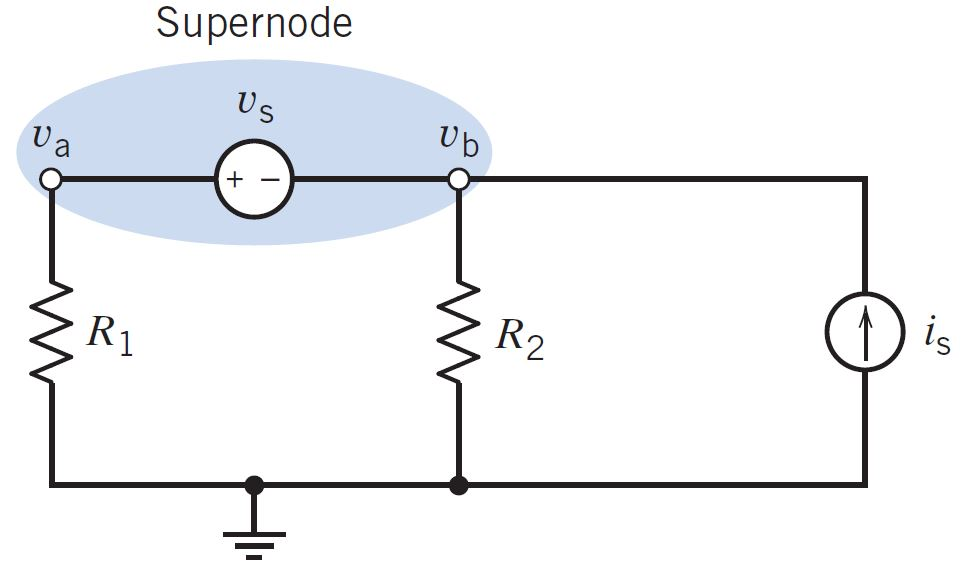
\includegraphics[width=.9\textwidth]{figura4_23.jpg}\\	
	%	\scalebox{1}{Answer:$\ v_{a} = -4/3V\ and \  v_{b} = 4 V$}
		\end{column}
		\begin{column}{0.4\textwidth}  %%<--- here
			\begin{equation}
			 v_{a}-v_{b}= v_{s}\ or \ v_{a}=v_{s}+ v_{b}
			\end{equation}
			\begin{equation}
			- i_{s}+\frac{ v_{b}}{R_{2}}+\frac{ v_{a}}{R_{1}}=0
			\end{equation}
			\begin{equation}
			- i_{s}+\frac{ v_{b}}{R_{2}}+\frac{ v_{s}+ v_{b}}{R_{1}}=0
			\end{equation}
			\begin{equation}
			 v_{b}=\frac{ R_{1}R_{2}i_{s}+R_{2}v_{s}}{R_{1}+R_{2}}
			\end{equation}
		\end{column}
	\end{columns}\\

	\begin{columns}[c]	\column{1\textwidth}
		A supernode consists of two nodes connected by an independent or a dependent voltage source.
	\end{columns} 
\end{tabular}
\end{frame}

% ----------------- NOVO SLIDE --------------------------------
\begin{frame}[fragile]
	\frametitle{Node Equations}

\begin{tabular}{ll}
	\begin{columns}
		\begin{column}{1\textwidth}  %%<--- here
		\textbf{EXAMPLE 4.3-2} - Determine the values of the node voltages $v_{a}$ and $v_{b}$ for the circuit.\\
		\begin{center}
    			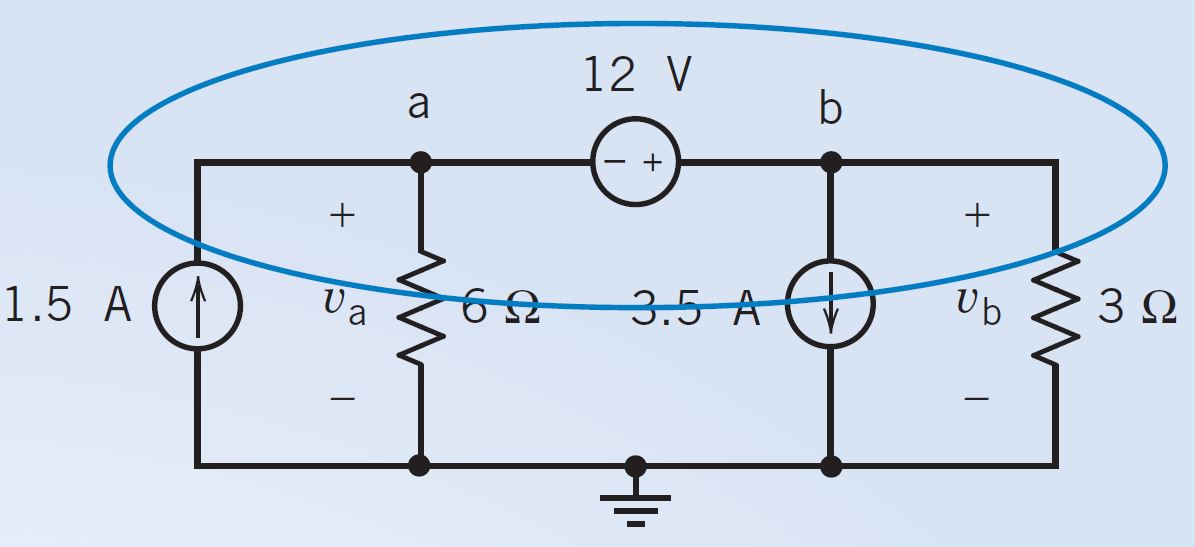
\includegraphics[width=.6\textwidth]{figura4_36.jpg}\\	
		\end{center}	
		\scalebox{0.8}{Answer:$\ v_{a} = -12V\ and \  v_{b} = 0 V$}
		\end{column}
	\end{columns}
\end{tabular}
\end{frame}
% ----------------- NOVO SLIDE --------------------------------
\begin{frame}[fragile]
	\frametitle{Node Equations}

\begin{tabular}{ll}
	\begin{columns}
		\begin{column}{1\textwidth}  %%<--- here
		\textbf{EXAMPLE 4.3-3} - Determine the node voltages for the circuit shown.\\
		\begin{center}
    			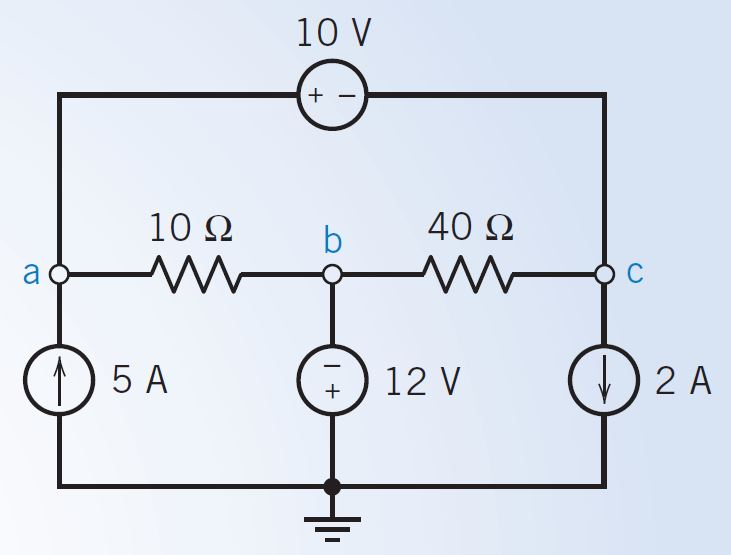
\includegraphics[width=.35\textwidth]{figura4_37.jpg}\\	
		\end{center}	
		\scalebox{0.8}{Answer:$\ v_{a} = 14V\ v_{b} = -12V\ and \  v_{c} = 4V$}
		\end{column}
	\end{columns}
\end{tabular}
\end{frame}
% ----------------- NOVO SLIDE --------------------------------
\begin{frame}[fragile]
	\frametitle{Node Equations}

\begin{tabular}{ll}
	\begin{columns}
		\begin{column}{1\textwidth}  %%<--- here
		\textbf{EXERCISE 4.3-2} - Find the voltages  $v_{a}$ and  $v_{b}$ for the circuit.\\
		\begin{center}
    			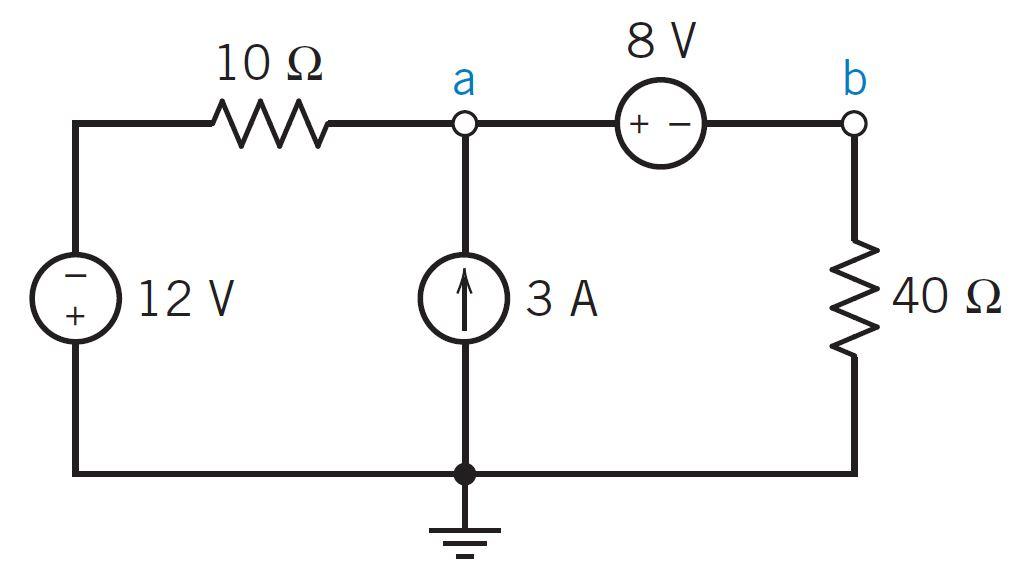
\includegraphics[width=.5\textwidth]{figuraE4_32.jpg}\\	
		\end{center}	
		\scalebox{0.8}{Answer:$\ v_{a} = 16V\ and \  v_{b} = 8V$}
		\end{column}
	\end{columns}
\end{tabular}
\end{frame}
% ----------------- NOVA SECÇÂO -----------------------------
\section{Node Voltage Analysis with Dependent Sources (4.4)}
% ----------------- NOVO SLIDE --------------------------------
\begin{frame}[fragile]
	\frametitle{Node Voltage Analysis with Dependent Sources}

\begin{tabular}{ll}
	\begin{columns}[c]	\column{1\textwidth}
		When a circuit contains a dependent source the controlling current or voltage of that
dependent source must be expressed as a function of the node voltages.
	\end{columns} \\
	\begin{columns}
		\begin{column}{0.5\textwidth}  %%<--- here
		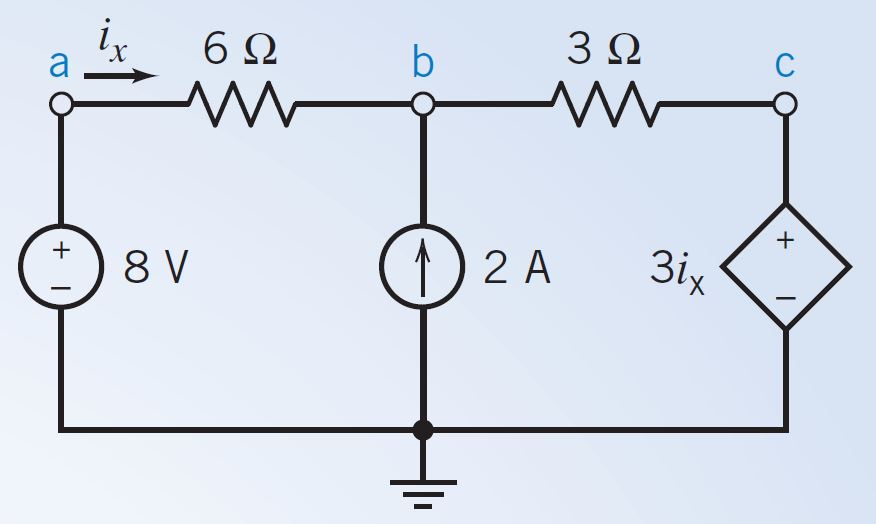
\includegraphics[width=.9\textwidth]{figura4_41.jpg}\\	
	%	\scalebox{1}{Answer:$\ v_{a} = -4/3V\ and \  v_{b} = 4 V$}
		\end{column}
		\begin{column}{0.5\textwidth}  %%<--- here
			\begin{equation}
			 i_{x}=\frac{v_{a}-v_{b}}{6}=\frac{8-v_{b}}{6}
			\end{equation}
			\begin{equation}
			v_{c}=3i_{x}=3(\frac{8-v_{b}}{6})
			\end{equation}
			\begin{equation}
			-\frac{v_{a}-v_{b}}{6}-2-\frac{v_{c}-v_{b}}{3}=0
			\end{equation}
			\begin{equation}
			-\frac{8-v_{b}}{6}-2-\frac{3(\frac{8-v_{b}}{6})-v_{b}}{3}=0
			\end{equation}
		\end{column}
	\end{columns}\\

	\begin{columns}[c]	\column{1\textwidth}
		A supernode consists of two nodes connected by an independent or a dependent voltage source.\
\scalebox{0.8}{Answer:$\ v_{a} = 8V, v_{b}=7V\ and \  v_{c} = \frac{1}{2}V$}
	\end{columns} 
\end{tabular}
\end{frame}

% ----------------- NOVO SLIDE --------------------------------
\begin{frame}[fragile]
	\frametitle{Node Equations}

\begin{tabular}{ll}
	\begin{columns}
		\begin{column}{1\textwidth}  %%<--- here
		\textbf{EXERCISE 4.4-1} - Find the node voltage $v_{b}$ for the circuit shown.\\
		\begin{center}
    			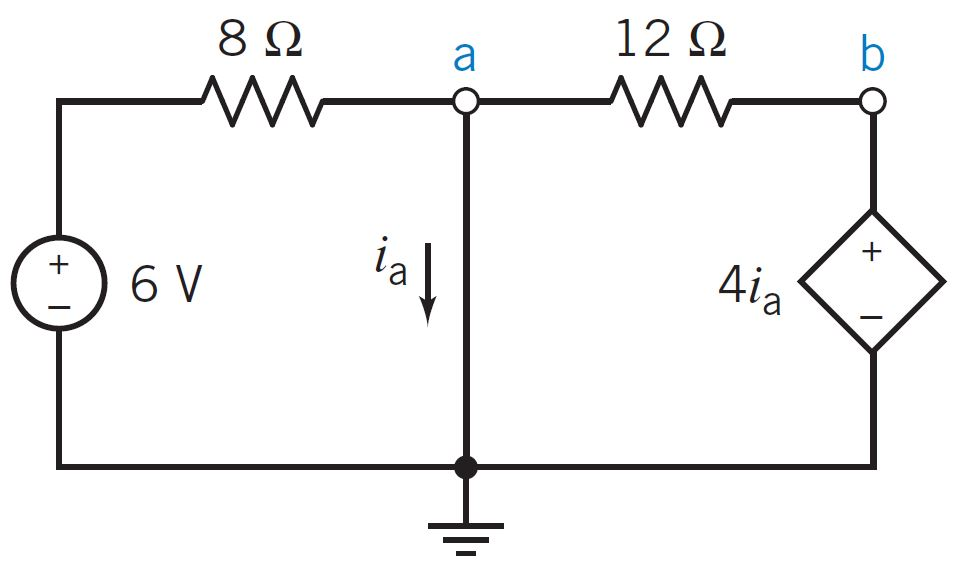
\includegraphics[width=.45\textwidth]{figuraE4_41.jpg}\\	
		\end{center}	
		\scalebox{0.8}{Answer: $ v_{b} = 4.5V$}
		\end{column}
	\end{columns}
\end{tabular}
\end{frame}


% ----------------- NOVA SECÇÂO -----------------------------
\section{Circuit Analysis Using MATLAB (4.9)}
% ----------------- NOVO SLIDE --------------------------------
\begin{frame}[fragile]
	\frametitle{ Circuit Analysis Using MATLAB}


\begin{tabular}{ll}
	\begin{columns}[c]	\column{1\textwidth}
		In this section, we will use the MATLAB computer program to solve the equations.
	\end{columns} \\
	\begin{columns}
		\begin{column}{0.4\textwidth}  %%<--- here
		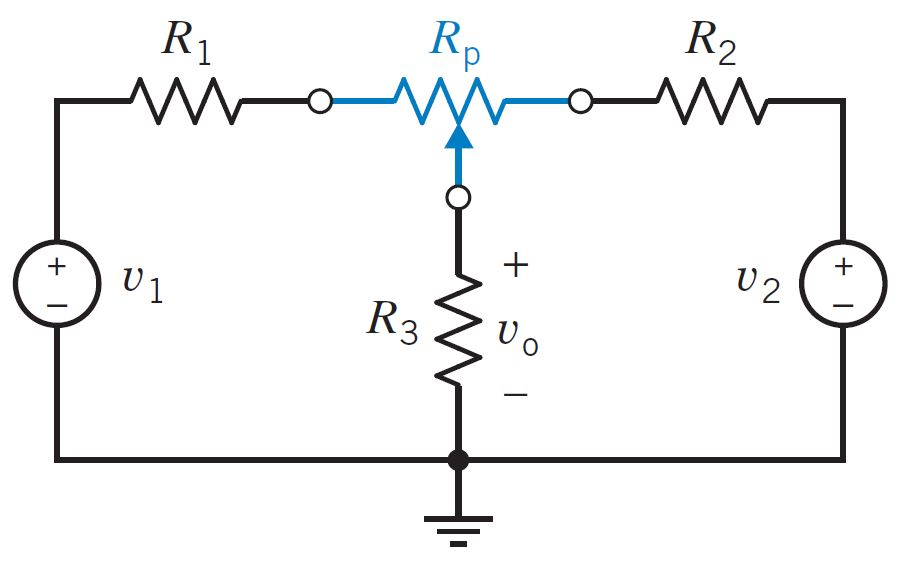
\includegraphics[width=1\textwidth]{figura4_91.jpg}\\	

		\scalebox{.6}{$\ R_{1} = 1000\Omega, \  R_{2} = 1000\Omega, \ R_{3}=5000\Omega, \ v_{1}=-v_{2}=15 V \ and \ R_{p}=20.000 \Omega$}
		\end{column}
		\begin{column}{0.6\textwidth}  %%<--- here
		{We have seen that circuits that contain resistors and independent or dependent sources can be analyzed
in the following way:}\\

					\begin{itemize}
						\item[$\clubsuit$] {Writing a set of node equations.}
						\item[$\clubsuit$]  {Solving those equations simultaneously.}
						
					\end{itemize}
		\end{column}
	\end{columns}
\end{tabular}



\end{frame}



\end{document} 